\section{Trial Space of Hyperparameter Tuning}

\begin{figure}[!h]
    \centering
    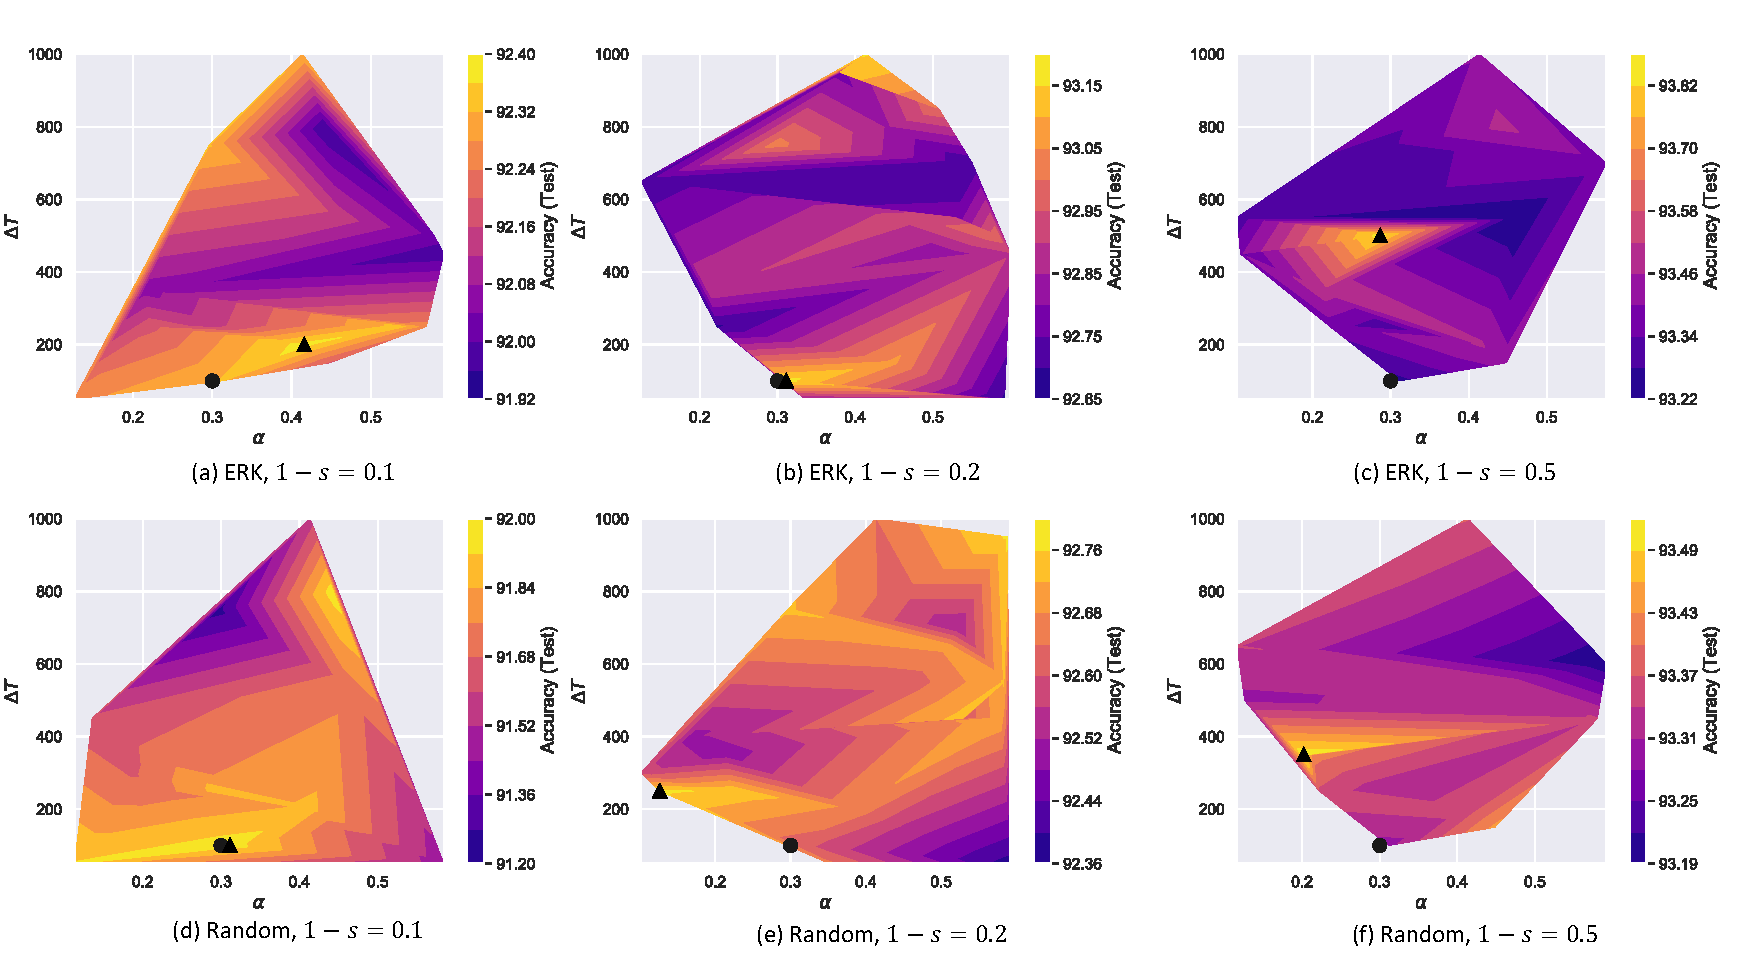
\includegraphics[width=\textwidth]{../openreview/supplementary_sections/alpha_delta_contour.pdf}
    \captionsetup{aboveskip=\figureaboveskip,belowskip=\figurebelowskip}
    \caption{\textbf{Trial space of tuning $(\alpha, \Delta T)$}, shown as a countor plot. Here, black circle corresponds to $(\alpha=0.3,\Delta T = 100)$, while black triangle corresponds to the optimal hyper-parameter pair found. We plot the convex hull of the trial space, so in a few cases the reference point lies on the border of this space.}
    \label{fig:alpha-deltaT-contour}
\end{figure}

Figure \ref{fig:alpha-deltaT-contour} shows the hyper-parameter study for tuning $(\alpha, \Delta T)$ as a contour plot. We observe that for multiple initialization-density configurations, the reference choice $(\alpha=0.3,\Delta T = 100)$, is quite close to the optimal hyper-parameters. Furthermore, where they differ, the difference is within standard deviation bounds (Table 4 of the main report).